\begin{figure}[htbp]
\centering
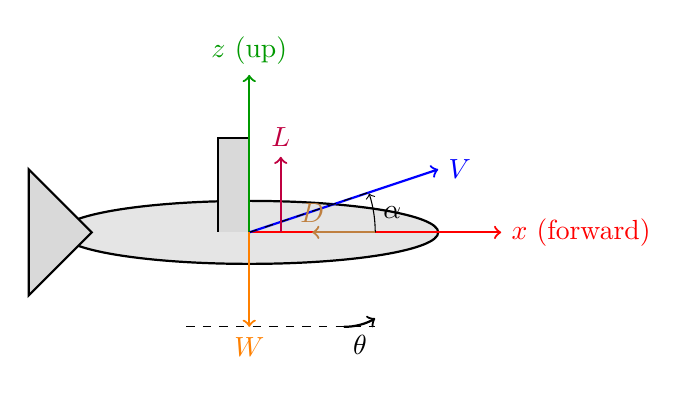
\begin{tikzpicture}[scale=0.8]
    % Aircraft body
    \draw[thick, fill=gray!20] (0,0) ellipse (3 and 0.5);
    \draw[thick, fill=gray!30] (-2.5,0) -- (-3.5,1) -- (-3.5,-1) -- cycle;
    \draw[thick, fill=gray!30] (0,0) -- (0,1.5) -- (-0.5,1.5) -- (-0.5,0);

    % Axes
    \draw[->, thick, red] (0,0) -- (4,0) node[right] {$x$ (forward)};
    \draw[->, thick, green!60!black] (0,0) -- (0,2.5) node[above] {$z$ (up)};

    % Velocity vector
    \draw[->, thick, blue] (0,0) -- (3,1) node[right] {$V$};

    % Angles
    \draw[->] (2,0) arc (0:18:2) node[midway, right] {$\alpha$};
    \draw[dashed] (0,0) -- (2,0.67);

    % Pitch angle
    \draw[->, thick] (1.5,-1.5) arc (-90:-60:1) node[midway, below] {$\theta$};
    \draw[dashed] (-1,-1.5) -- (2,-1.5);

    % Forces
    \draw[->, thick, orange] (0,0) -- (0,-1.5) node[below] {$W$};
    \draw[->, thick, purple] (0.5,0) -- (0.5,1.2) node[above] {$L$};
    \draw[->, thick, brown] (2,0) -- (1,0) node[above] {$D$};
\end{tikzpicture}
\caption{Aircraft longitudinal plane showing forces and angles.}
\label{fig:aircraft_longitudinal}
\end{figure}
